\subsection{Types of SPADs}\label{ssec:SPADs}
In Hazard Detection Mode, individual SPADs will have the responsibility of measuring their part in the target. Therefore it is important to first investigate what type of SPAD is best suited for the device. As mentioned in \cref{ssec:optics}, SPADs can have microlenses. Two types are considered: conventional spherical lenses, and rectangular lenses. Spherical lenses typically achieve an effective active area of approximately $55\,\%$, while rectangular lenses typically get an effective active area of appeoximately $65\,\%$. The active area can also be shaped in different sizes, and a circular and rectangular shape are considered here. An overview of the different options is shown in \cref{tkz:SPAD_types}.


\begin{figure}[H]
    \centering

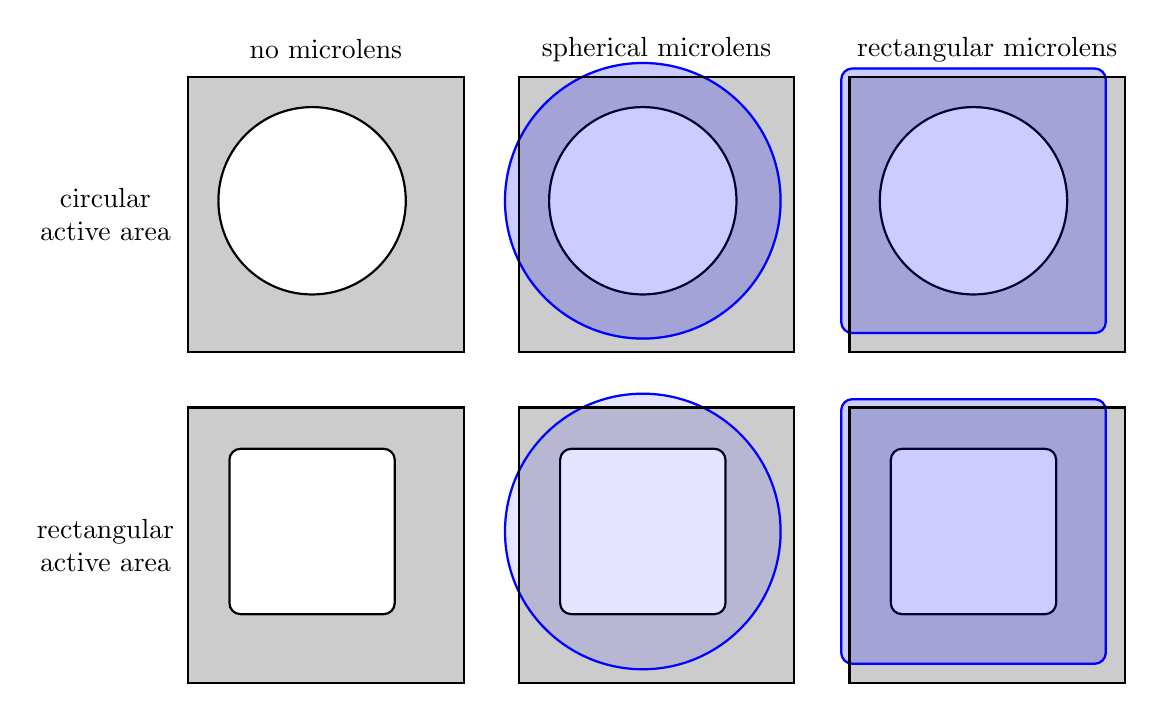
\begin{tikzpicture}[thick,scale=0.7, every node/.style={scale=1}]

\draw[fill, color=black!20]  (-1.25,3.25) rectangle (3.75,-1.75);
\draw[fill, color=white]  (1,1) ellipse (1.7 and 1.7);
\draw[]  (1,1) ellipse (1.7 and 1.7);

\draw[fill, color=black!20]  (4.75,3.25) rectangle (9.75,-1.75);
\draw[fill, color=white]  (7,1) ellipse (1.7 and 1.7);
\draw[]  (7,1) ellipse (1.7 and 1.7);
\draw [fill, color=blue, opacity=0.2] (7,1) ellipse (2.5 and 2.5);
\draw [color=blue] (7,1) ellipse (2.5 and 2.5);

\draw[fill, color=black!20]  (10.75,3.25) rectangle (15.75,-1.75);
\draw[fill, color=white]  (13,1) ellipse (1.7 and 1.7);
\draw[]  (13,1) ellipse (1.7 and 1.7);
\draw [fill, color=blue, opacity=0.2, rounded corners] (10.6,3.4) rectangle (15.4,-1.4);
\draw [color=blue, rounded corners] (10.6,3.4) rectangle (15.4,-1.4);

\draw[fill, color=black!20]  (-1.25,-2.75) rectangle (3.75,-7.75);
\draw[fill, color=white, rounded corners] (-0.5,-3.5) rectangle (2.5,-6.5) {};
\draw[rounded corners] (-0.5,-3.5) rectangle (2.5,-6.5) {};

\draw[fill, color=black!20]  (4.75,-2.75) rectangle (9.75,-7.75);
\draw[fill, color=white, rounded corners] (5.5,-3.5) rectangle (8.5,-6.5) {};
\draw[rounded corners] (5.5,-3.5) rectangle (8.5,-6.5) {};
\draw [fill, color=blue, opacity=0.1] (7,-5) ellipse (2.5 and 2.5);
\draw [color=blue] (7,-5) ellipse (2.5 and 2.5);

\draw[fill, color=black!20]  (10.75,-2.75) rectangle (15.75,-7.75);
\draw[fill, color=white, rounded corners] (11.5,-3.5) rectangle (14.5,-6.5) {};
\draw[rounded corners] (11.5,-3.5) rectangle (14.5,-6.5) {};
\draw [fill, color=blue, opacity=0.2, rounded corners] (10.6,-2.6) rectangle (15.4,-7.4);
\draw [color=blue, rounded corners] (10.6,-2.6) rectangle (15.4,-7.4);

\draw[]  (-1.25,3.25) rectangle (3.75,-1.75);
\draw[]  (4.75,3.25) rectangle (9.75,-1.75);
\draw[]  (10.75,3.25) rectangle (15.75,-1.75);

\draw[]  (-1.25,-2.75) rectangle (3.75,-7.75);
\draw[]  (4.75,-2.75) rectangle (9.75,-7.75);
\draw[]  (10.75,-2.75) rectangle (15.75,-7.75);

\node at (1.25,3.75) {no microlens};
\node at (7.25,3.75) {spherical microlens};
\node at (13.25,3.75) {rectangular microlens};
\node[align=center] at (-2.75,0.75) {circular\\active area};
\node[align=center] at (-2.75,-5.25) {rectangular\\active area};
\end{tikzpicture}
    \caption{Options for lenses with varying types of active areas and microlenses}
    \label{tkz:SPAD_types}
\end{figure}


The use of microlenses is not the only viable of option of increasing the active area on the chip. A second option is to pick the circuitry required per SPAD, and push it to the side. These circuitry include the Read-Out Integrated Circuit (ROIC) that also includes the quenching of the SPADs, and the Time interval to Digital converter (TDC). 

To avoid pileup, the following calculations are done for an $0.18\,\mu m$ technology and it is assumed that the ROIC will take up $110\,\mu m^2$ surface area per SPAD, and that the TDC will take up $1200\,\mu m^2$ surface area per SPAD. It will also be assumed that the minimum amount of pitch between two SPADs is $1.5\,\mu m$. These numbers are based on current SPAD designs in $0.18\,\mu m$ technology. An overview of the performance of all different possibilities is shown in \cref{fig:effective_area}.

\begin{figure}[h]
\centering
	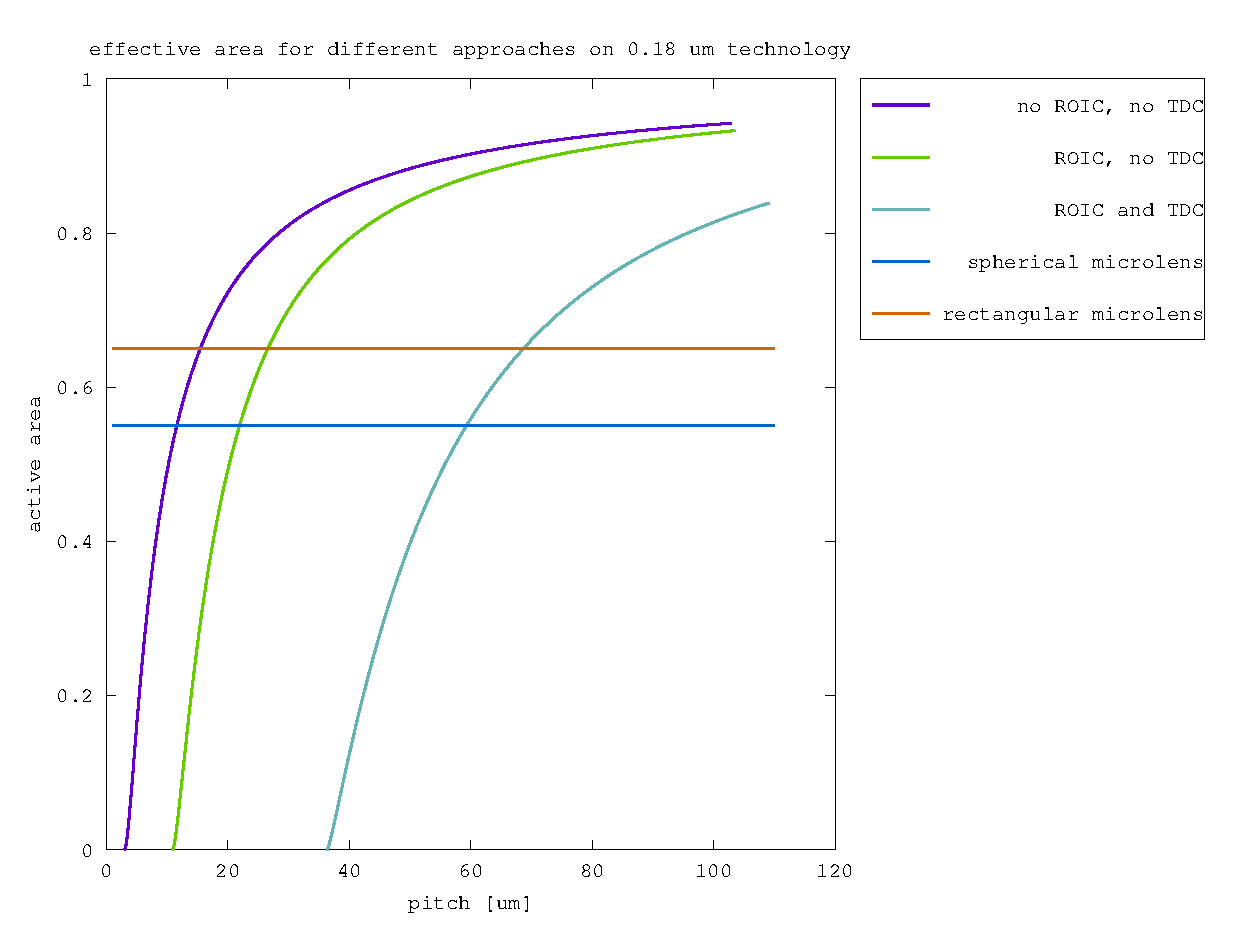
\includegraphics[width=0.8\linewidth]{fig/effective_area.eps}
\caption{effective area for different approaches in relationship to the pitch of the SPAD on $0.18\,\mu m$ technology}
\label{fig:effective_area}
\end{figure} 

